\clearpage
\section{}
Sprawdzono odpowiedź układu różniczkującego na falę prostokątną o okresie \(T\) mniejszym, porównywalnym i większym od stałej czasowej.
Zaobserwowano odpowiedź układu sygnał trójkątny.

\begin{figure}[H]
	\centering
	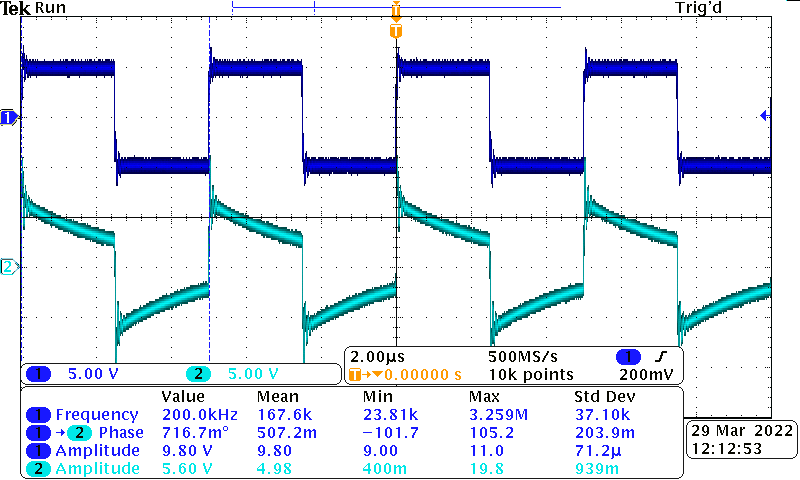
\includegraphics[width=\textwidth]{include/2/200_sq.png}
	\caption{Obserwacja odpowiedzi układu na falę prostokątną o \(f=200\)kHz}
\end{figure}
\begin{figure}[H]
	\centering
	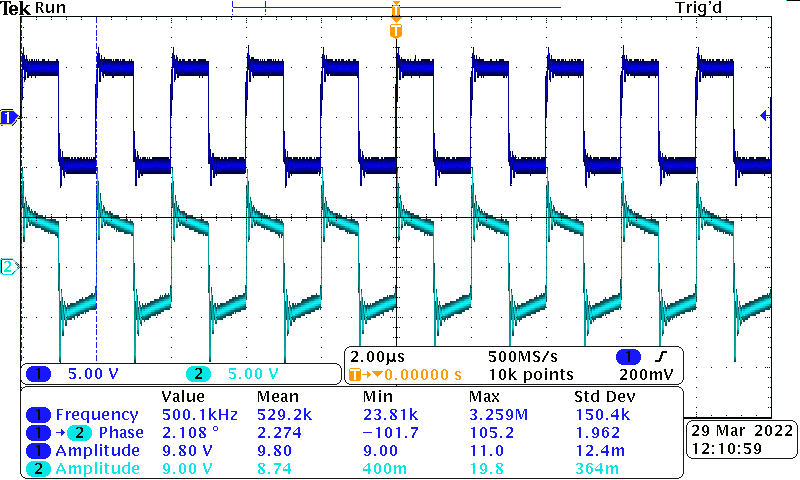
\includegraphics[width=\textwidth]{include/2/500_sq.png}
	\caption{Obserwacja odpowiedzi układu na falę prostokątną o \(f=500\)kHz}
\end{figure}
\begin{figure}[H]
	\centering
	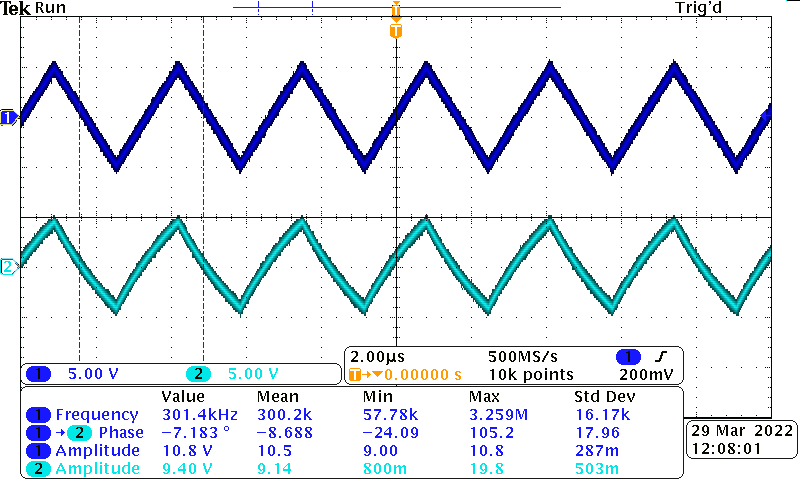
\includegraphics[width=\textwidth]{include/2/nom_tr.png}
	\caption{Obserwacja odpowiedzi układu na falę trójkątną o \(f=300\)kHz}
\end{figure}
